\documentclass[../main.tex]{subfiles}
\graphicspath{ {../img/} }


\begin{document}


	\chapter{Code analysis and difficulties.}


	\section{Why Rust?}


    Rust is a multi-paradigm low level programming language which emphasizes memory safety, strict types and high performance. 
    Despite its novel features(and associated learning curve), such as variable ownership and its ommission of a null variable, it is already a loved language among developers, which forces the developer to write safer and more performant code.
    Despite it lacking as many footguns as C/C++, it allows a great deal of control over what happens in a program. 
    Though young, Rust is seen as the spearhead for the languages of the future, looking to replace C++ as the dominant low level language. 
    Rust has been added to the Linux kernel, currently the only language to accompany C in this domain, and is being picked up by even the largest companies, such as Google. On the opposite side of the spectrum, hackers have begun writing in Rust, due to its aforementioned strengths and the current inability for malware scanners to detect threats in the binary[reference]. 
    All of these reasons combined form our argument for learning Rust, which is what we had to do for this project.

	\vspace{10pt}

	\section{Flow of the program}

    Let's Now analyse our rust code to have a better understading of the communications in our botnet.
	\vspace{10pt}

	\subsection{Server code}

    \# server/src/main.rs

    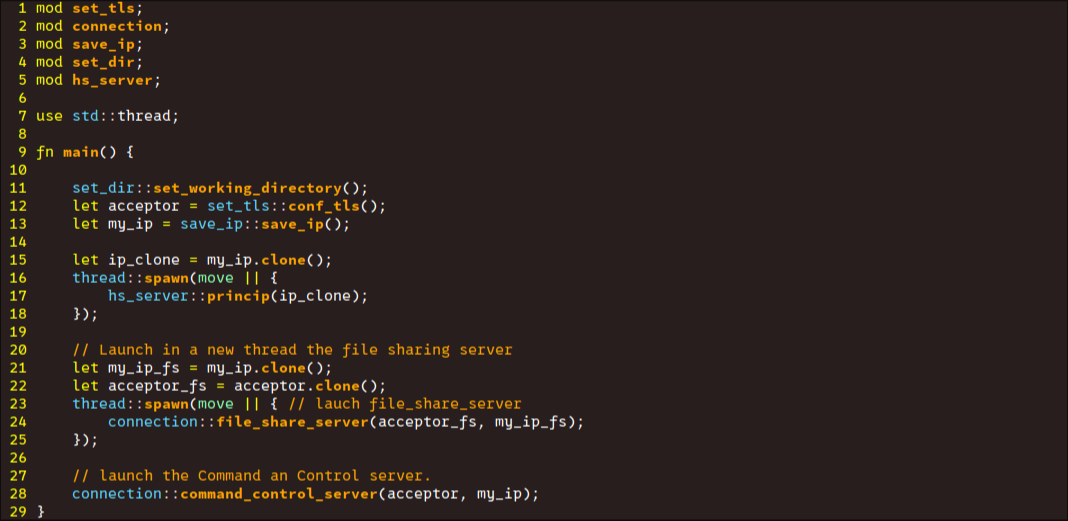
\includegraphics[width=450pt]{server_main.png}

    Firstl, we import different modules that we have written on line 1-5 , to modularize and simplify the code.
    Then, at line 7, we import thread.
    The main function begins and we set the working directory to where the binary is.
    After that, we create the acceptor, save the server ip address, and create a new thread for hs\_server, the hacking server, which will transform the victim into a bot.
    Now, we are approaching the last part of the server.
    We create a thread for the file sharing server in wich the file sharing server is called and wait for connection to launch command and control server.

    
	\vspace{10pt}

	\subsection{Client code}

    Now, let's talk about the client's code.

    \# client/src/main.rs

    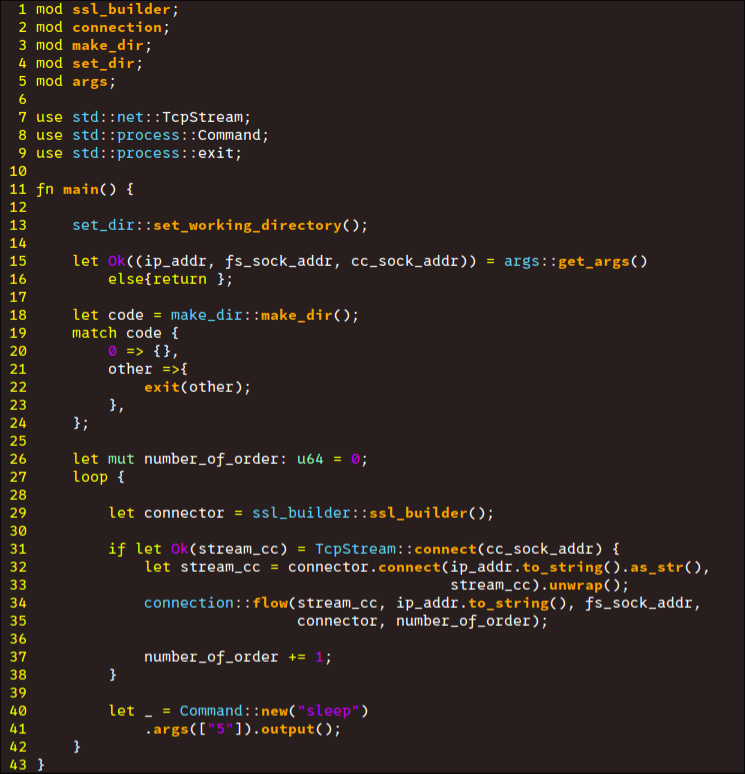
\includegraphics[width=450pt]{client_main.png}

    At the begining of the main it imports the different functions.
    Then it imports TcpStream, command, and exit, to make the stream object, run system commands and to exit in case there is a problem.
    Then, at the beginning of the main function, the working directory is set to where the binary is, it makes all the necessary directory ie. www, downloaded, conf, and exits in case of an error.
    Then, it makes the stream with the CC server, and launches the flow function. 
    It counts the number of times it loops, which also informs how many times it connected to the server, then it asks for order1 or order2 in the flow function.
    After each successful connection it waits for 5 seconds before launching the next connection.

    \# client/src/connection.rs

    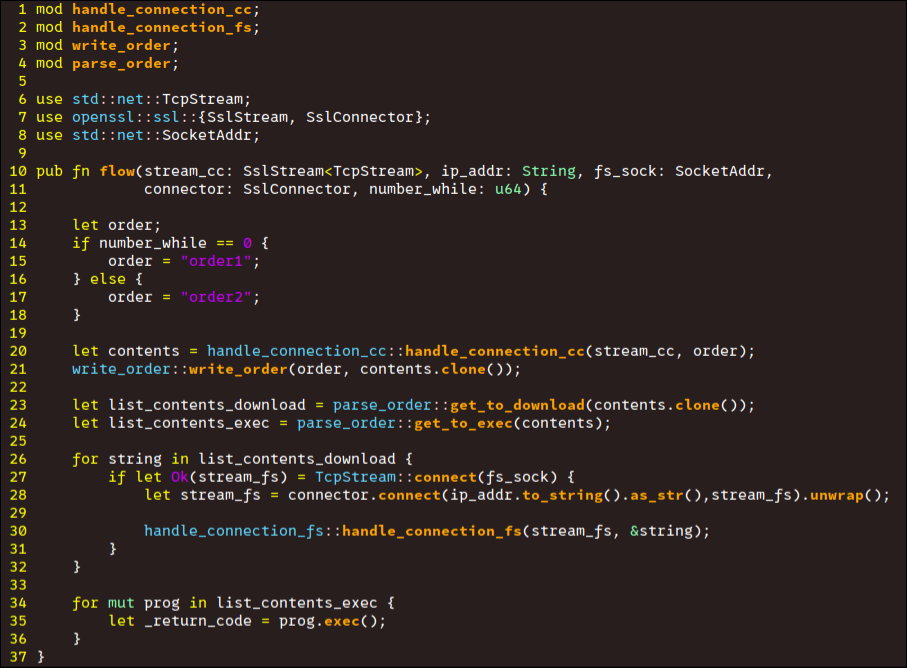
\includegraphics[width=450pt]{client_flow.png}

    This is the flow function.
    First, it determines if it has to ask for the installation order or the attack order depending on how many times it has looped.
    Then it requests it's order from the CC server, parses it, and makes a list of files to download and of files to execute.
    After that, for each item to downloaded, it makes a connection with the filesharing server to download it, and after downloaded all the necessary files, it executes all the files recieved.
    Usually this is just a BASH script.


	\vspace{10pt}

	\section{Difficulties encountered while writing the program}

    While writing our botnet's code, we encountered a variety of difficulties.
    Firstly, it was the first time we were coding in rust, so we had to learn the language.
    Secondly, it was just the three of us doing the project, we needed to be well organised and to distribute our tasks.
    We also had problems with the code;
    For instance, we first chose Openssl as our tls library but we find out that we needed to build statically linked binaries in order to make them run on the victim, and so for that we had to use musl and rustls.
    This we could put on for the server, but because we were using self signed certificates, we had to keep Openssl for the client.
    The solution we found for the client was to active the cross-compilation for OpenSsl, and the problem was solved.
    We also encountered other difficulties because of the cross-compilation.
    For exmaple we found that our exploit was using curl, so we tried to build it statically linked, but we failed, so we looked for an already statically linked binary of curl on the internet, which we thankfully found.
    Our original client design had a big flow in it, and so we had to rewrite again all the main and flow function.
    Fortunately, it was only thoses two function that had to be rewritten.



\end{document}
